% !TeX root = ../../main.tex
\section{Zbiory danych}
\label{sec:zbiory}
Do przeprowadzenia eksperymentów (Rozdział \numberref{sec:eksperymenty_wyniki}) skonstruowano dwa zbiory danych, w skład których wchodzą m.in. obrazy otrzymane od firmy \blue{}, wykonane w różnych ośrodkach sportowych.
Jeden zbiór, zwany dalej zbiorem \textit{low}, pochodzi z~kamer usytuowanych na podłodze, tuż przy liniach kortu. Obrazy w zbiorze \textit{low} są monochromatyczne oraz tej samej rozdzielczości.
Drugi zbiór, zwany dalej zbiorem \textit{high} pochodzi z~kamer ustawianych w większej odległości od kortu oraz na wyższej wysokości w~porównaniu do zbioru \textit{low}. Zdjęcia w zbiorze \textit{high} są kolorowe i nie charakteryzują się jednakową rozdzielczością.


\begin{figure}[!htb]
  \minipage{0.45\textwidth}
    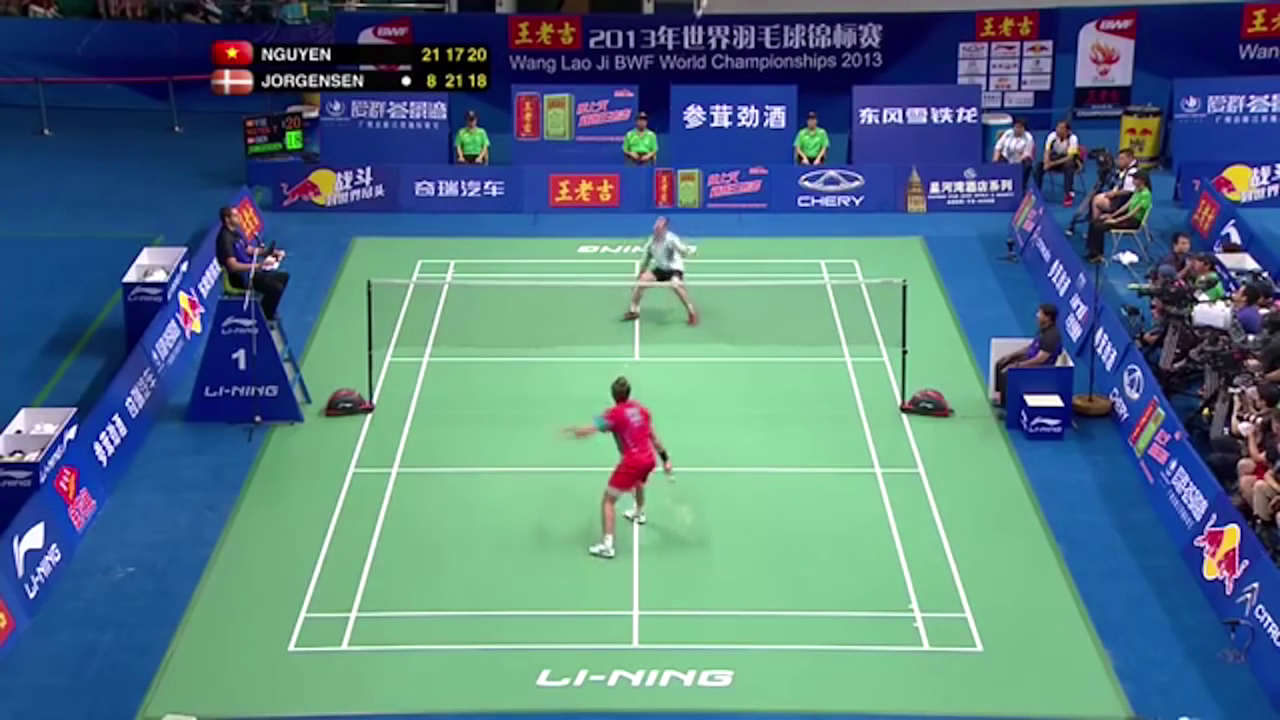
\includegraphics[width=\linewidth]{../../badminton/datasets/high/split/test_court2-00002.png}
    \caption{Przykładowy obraz ze zbioru danych \textit{high} o rozdzielczości 1280x720~pikseli}
  \endminipage\hfill
  \minipage{0.45\textwidth}
    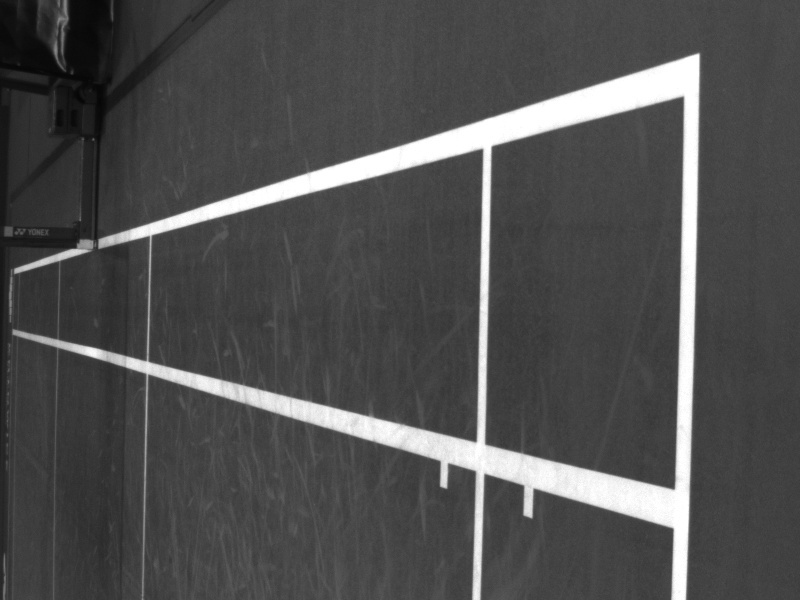
\includegraphics[width=\linewidth]{../../badminton/datasets/low/split/1564909032792410075.jpg}
    \caption{Przykładowy obraz ze zbioru danych \textit{low} o rozdzielczości 896x640~pikseli}
  \endminipage\hfill
\end{figure}

Zbiór \textit{low} zawiera wyłącznie monochromatyczne obrazy o rozdzielczości 896x640 pikseli pozyskane od firmy \blue{}. Obrazy te pochodzą z kamer ustawianych od 50 do 120 centymentrów nad ziemią, w odległości od 75 do 350 centymentrów od najbliższej linii kortu.

\begin{table}[!h]
	\centering
	\caption{Liczność zbiorów danych}
	\vspace{6pt}
	{\footnotesize
		\begin{tabular}{|c|c|c|c|}
			\hline \textbackslash & Liczność & Rozdzielczość & Kolor \\
      \hline Zbiór \textit{low} & 207 & 896x640 & monochromatyczny \\
      \hline Zbiór \textit{high} & 97 & od 259x194 do 1280x720 & polichromatyczny \\
      \hline
    \end{tabular}
    \label{Tab:licznosc}
	}
	\vspace{0pt}
\end{table}

Zbiór danych \textit{high} składa się z 36 obrazów o wymiarach 1280x720 pikseli, 6 obrazów o rozdzielczości 480x360, 4 obrazów o rozdzielczości 640x480, i pozostałych obrazów o różnych rozdzielczościach, od 259x194 pikseli do 2040x1530 pikseli. Obrazy pochodzą z~różnych źródeł - od firmy \blue{}, z~Internetu (z serwisu \textit{Google Images}) oraz ze~zrzutów ekranu transmisji zawodów sportowych. Sumaryczna liczność elementów w zbiorach danych przedstawiona jest w~Tabeli \mytabref{Tab:licznosc}.

\subsection{Podzbiór treningowy, walidacyjny i testowy}
\label{sec:podzial}
W tym rozdziale omówiono podział zbiorów danych na podzbiory treningowe, walidacyjne i testowe.
Ze względu na stosunkowo małą liczność zbiorów danych, podzbiór testowy został ograniczony do dwóch obrazów.
Pozostałe obrazy, wchodzące w skład podzbiorów treningowych i walidacyjnych zostały rozdzielone w różny sposób, tak aby umożliwić przeprowadzenie eksperymentów w celu wybrania podziału dającego możliwie jak najlepsze wyniki.
Podział zbiorów danych przedstawiono w~Tabeli \mytabref{Tab:podzial}.

\begin{table}[H]
	\centering
	\caption{Liczba obrazów w podziale na poszczególne podzbiory danych.}
	\vspace{6pt}
	{
    \footnotesize
    \begin{tabular}{|c|c|c|c|}
      \hline \textbackslash & Podzbiór treningowy & Podzbiór walidacyjny & Podzbiór testowy \\
      \hline Zbiór \textit{high\_92\_5} & 92 (94.85\%) & 5 (5.15\%) & 2 (2.06\%) \\
      \hline Zbiór \textit{high\_87\_10} & 87 (89.69\%) & 10 (10.31\%) & 2 (2.06\%) \\
      \hline Zbiór \textit{high\_73\_24} & 73 (75.26\%) & 24 (24.74\%) & 2 (2.06\%) \\
      \hline Zbiór \textit{high\_49\_48} & 49 (50.52\%) & 48 (49.48\%) & 2 (2.06\%) \\
      \hline
      \hline Zbiór \textit{low\_197\_10} & 197 (95.17\%) & 10 (4.83\%) & 2 (0.97\%) \\
      \hline Zbiór \textit{low\_186\_21} & 186 (89.86\%) & 21 (10.14\%) & 2 (0.97\%) \\
      \hline Zbiór \textit{low\_155\_52} & 155 (74.88\%) & 52 (25.12\%) & 2 (0.97\%) \\
      \hline Zbiór \textit{low\_104\_103} & 104 (50.24\%) & 103 (49.76\%) & 2 (0.97\%) \\
      \hline
    \end{tabular}
    \label{Tab:podzial}
	}
	\vspace{0pt}
\end{table}

W~Tabeli \mytabref{Tab:podzial} w nawiasach zaznaczono procentowy udział danego podzbioru w stosunku do całego zbioru.
